%% LyX 2.4.2.1 created this file.  For more info, see https://www.lyx.org/.
%% Do not edit unless you really know what you are doing.
\documentclass[12pt,twoside,twocolumn,spanish]{Plantilla}
\usepackage[T1]{fontenc}
\usepackage[latin9]{inputenc}
\setcounter{secnumdepth}{5}
\setcounter{tocdepth}{3}
\usepackage{babel}
\addto\shorthandsspanish{\spanishdeactivate{~<>}}
\deactivatequoting

\usepackage{pifont}
\usepackage{float}
\usepackage{amsmath}
\usepackage{graphicx}
\usepackage[paperwidth=30cm,paperheight=39cm]{geometry}
\geometry{verbose,tmargin=5cm,bmargin=3cm,lmargin=3cm,rmargin=3cm,columnsep=1cm}
\usepackage[authoryear]{natbib}
\usepackage[unicode=true,pdfusetitle,
 bookmarks=true,bookmarksnumbered=false,bookmarksopen=false,
 breaklinks=false,pdfborder={0 0 0},pdfborderstyle={},backref=false,colorlinks=false]
 {hyperref}

\makeatletter

%%%%%%%%%%%%%%%%%%%%%%%%%%%%%% LyX specific LaTeX commands.
%% Because html converters don't know tabularnewline
\providecommand{\tabularnewline}{\\}

%%%%%%%%%%%%%%%%%%%%%%%%%%%%%% User specified LaTeX commands.
\usepackage{Plantilla}

\AtBeginDocument{
  \def\labelitemi{\ding{109}}
  \def\labelitemii{\ding{113}}
  \def\labelitemiii{\Pisymbol{psy}{68}}
  \def\labelitemiv{\ding{226}}
}

\makeatother

\begin{document}

\Titulo{T�tulo del Art�culo}

\Autores{Nombre del Autor}

\AutoresCorto{Autor Corto}

\Correo{Correo del Autor}

\Materia{M�todos Num�ricos}

\Institucion{Universidad del Quind�o}

\Fecha{Mes y A�o}

\NombreCapitulo{Ca�da Libre}

\TipoCapitulo{Informe}

\NumeroArticulo{0}

\chapter{T�tulo del Informe}

\InformacionAutor{}

\section{Resumen}

Lorem ipsum dolor sit amet, consectetur adipiscing elit. Donec bibendum
velit vel pretium ultricies. Praesent vehicula felis vitae lacus bibendum
pharetra. Donec non odio feugiat, accumsan nunc vel, interdum purus.
Sed semper egestas nisl in ultrices. Curabitur facilisis felis vitae
odio egestas, eget pretium quam tempus. Suspendisse enim nisi, ullamcorper
semper augue id, volutpat facilisis mauris.\\


\section{Explicaci�n del Fen�meno o Modelo}

In tempus sapien massa, a interdum ipsum laoreet eget. Vivamus gravida
enim ex, porttitor ultricies augue pulvinar ut. Praesent sit amet
magna cursus, facilisis tellus ut, rhoncus nisl. Vivamus et lacinia
purus, quis vehicula leo. Nulla aliquam pulvinar odio id eleifend.
Interdum et malesuada fames ac ante ipsum primis in faucibus. Morbi
cursus ullamcorper augue in efficitur. Aliquam ullamcorper orci vel
erat commodo hendrerit. Proin eu semper lorem. Aenean leo lacus, gravida
vitae eleifend ac, luctus nec ante. \\

A continuaci�n se muestra una gr�fica de la funci�n.

\begin{figure}[H]
\begin{centering}
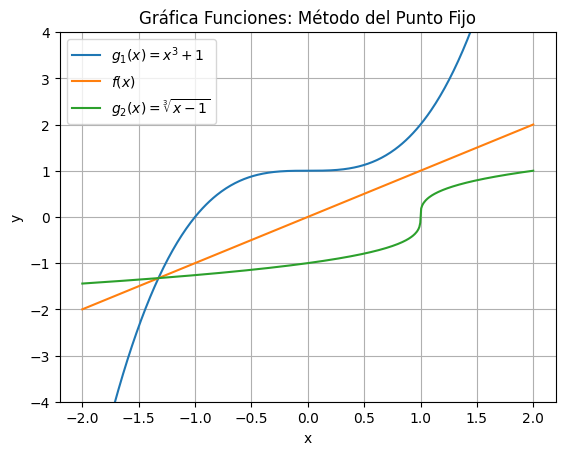
\includegraphics[width=12cm]{Imagenes/grafica-funciones}
\par\end{centering}
\caption{Etiqueta de la gr�fica}

\end{figure}

Tenemos un sistema de ecuaciones

\begin{equation}
S=\begin{cases}
ax+by & =c\\
dx+ey & =f
\end{cases}\label{eq:sistema-1}
\end{equation}


\section{Datos}

Se hace una recopilaci�n de los datos generados por el experimento
y se explica su procedencia y la forma de tomarlos.

Una tabla de datos del sistema \ref{eq:sistema-1}

\begin{table}[H]
\begin{centering}
\begin{tabular}{|c|c|}
\hline 
$x$ & $f\left(x\right)$\tabularnewline
\hline 
$1$ & $2$\tabularnewline
\hline 
$2$ & $3$\tabularnewline
\hline 
$3$ & $5$\tabularnewline
\hline 
$4$ & $7$\tabularnewline
\hline 
$5$ & $11$\tabularnewline
\hline 
\end{tabular}
\par\end{centering}
\caption{Etiqueta de la tabla}
\end{table}


\section{Pseudoc�digo}

Explicaci�n de los pasos necesarios para resolver el problema.

\section{C�digo en Python}

Explicaci�n y referencia del c�digo en Python, ya sea realizado en
Google Colab, Visual Studio, Spider, etc.\\

Para ello existe el comando Google Colab \citet{key-1}

\GoogleColab{https://colab.research.google.com/drive/1QSB8MEK27cfr3pHqCGi3tjCtGq-uiNyz?usp=sharing}{}

\begin{lstlisting}
# Crear un *programa* en **Python** que grafique el polinomio $P_{3}\left(x\right)=x^{3}-10x^{2}+6x-30$ para $x\in\left[1,6\right]$

# Importar las librerias necesarias
import numpy as np
import matplotlib.pyplot as plt

# Definir el polinomio
def poly(x):
    return x**3 - 10*x**2 + 31*x - 30

# Crear el dominio de graficaci�n
x = np.linspace(1, 6, 100)

# Evaluar el polinomio en x
y = poly(x)

# Graficar y configurar la gr�fica
plt.plot(x, y)
plt.xlabel('$x$')
plt.ylabel('$P_n(x)$')
plt.title('Gr�fico del Polinomio $P_n(x)$')
plt.grid(linestyle='--')
plt.show()
\end{lstlisting}

\section{Simulaciones}

Se muestran im�genes de las gr�ficas de las simulaciones y los respectivos
resultados.\\

\begin{figure}[H]
\begin{centering}
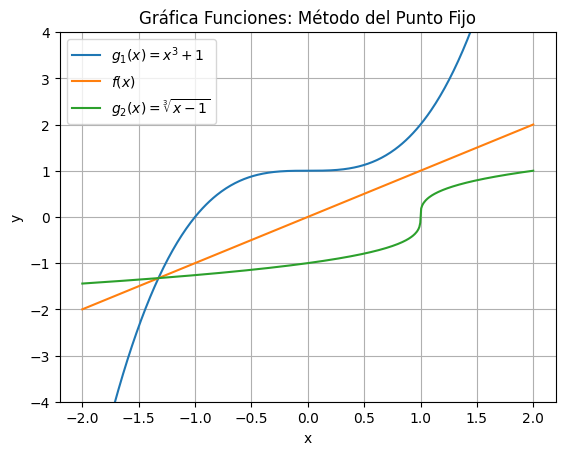
\includegraphics[width=12cm]{Imagenes/grafica-funciones}
\par\end{centering}
\caption{Etiqueta de la gr�fica}
\end{figure}


\section{An�lisis del M�todo}

Se debe mostrar el an�lisis de:
\begin{enumerate}
\item Convergencia
\item Velocidad de Convergencia
\item Error
\item M�todo (Cu�l es el m�todo m�s apropiado para resolver el problema)
\end{enumerate}

\section{Conclusiones}

Se generan las conclusiones al problema.
\begin{enumerate}
\item Conclusi�n 1
\item Conclusi�n 2
\item Conclusi�n 3
\end{enumerate}
\begin{thebibliography}{Rinc�n, J (2012)}
\bibitem[Rinc�n, J(2012)]{key-1} Rinc�n, J. (2012). \emph{Gr�fica
de funciones polares}. Editorial Elizcom

\bibitem{key-2}Rinc�n, J. (2012). \emph{Gr�fica de funciones polares}.
Editorial Elizcom

\bibitem{key-3}Rinc�n, J. (2012). \emph{Gr�fica de funciones polares}.
Editorial Elizcom

\end{thebibliography}

\end{document}
